% options:
% thesis=B bachelor's thesis
% thesis=M master's thesis
% czech thesis in Czech language
% english thesis in English language
% hidelinks remove colour boxes around hyperlinks

\documentclass[thesis=M,english]{FITthesis}[2019/12/23]

\usepackage[utf8]{inputenc} % LaTeX source encoded as UTF-8
% \usepackage[latin2]{inputenc} % LaTeX source encoded as ISO-8859-2
% \usepackage[cp1250]{inputenc} % LaTeX source encoded as Windows-1250

\usepackage{subfig} %subfigures
\usepackage{pdfpages}
\usepackage{amsmath} %advanced maths
\usepackage{amssymb} %additional math symbols
\usepackage{amsthm}
\usepackage{dirtree} %directory tree visualisation
\usepackage{todonotes}
\usepackage[outputdir=./tmp]{minted}
\usepackage{xcolor}

\newcommand{\tg}{\mathop{\mathrm{tg}}} %cesky tangens
\newcommand{\cotg}{\mathop{\mathrm{cotg}}} %cesky cotangens

% % list of acronyms
% \usepackage[acronym,nonumberlist,toc,numberedsection=autolabel]{glossaries}
% \iflanguage{czech}{\renewcommand*{\acronymname}{Seznam pou{\v z}it{\' y}ch zkratek}}{}
% \makeglossaries

% % % % % % % % % % % % % % % % % % % % % % % % % % % % % % 
% EDIT THIS
% % % % % % % % % % % % % % % % % % % % % % % % % % % % % % 

\nocite{*}

% \includeonly{
%  content/0-Introduction,
%  content/1-terminology,
%  content/2-framework-selection,
%  content/3-evaluation-criteria,
%  content/4-implementation
% }

\department{Department of Software Engineering}
\title{Object-relational mapping for database access in JavaScript}
\authorGN{Ladislav} %author's given name/names
\authorFN{Louka} %author's surname
\author{Ladislav Louka} %author's name without academic degrees
\authorWithDegrees{Bc. Ladislav Louka} %author's name with academic degrees
\supervisor{Ing. Jan Matoušek}
\acknowledgements{THANKS (remove entirely in case you do not with to thank anyone)}
\abstractEN{TODO Summarize the contents and contribution of your work in a few sentences in English language.}
\abstractCS{TODO}
\placeForDeclarationOfAuthenticity{Prague}
\keywordsCS{Replace with comma-separated list of keywords in Czech.}
\keywordsEN{Replace with comma-separated list of keywords in English.}
\declarationOfAuthenticityOption{1} %select as appropriate, according to the desired license (integer 1-6)
% \website{http://site.example/thesis} %optional thesis URL

\linespread{1.3}


\newtheorem{definition}{Definition}

\begin{document}

% \newacronym{CVUT}{{\v C}VUT}{{\v C}esk{\' e} vysok{\' e} u{\v c}en{\' i} technick{\' e} v Praze}
% \newacronym{FIT}{FIT}{Fakulta informa{\v c}n{\' i}ch technologi{\' i}}

\chapter{Introduction}

In the modern world, data have become an essential aspect of almost every field.
From e-commerce to healthcare, education to finance, data is everywhere and
plays a~critical role in decision-making processes. The advent of Web 2.0
\cite{Web2Oreilly}, which brought the concept of user-generated content, was
largely supported by connecting the Web to databases. Social media platforms,
for example, rely heavily on data to provide personalized recommendations,
targeted advertising, and other features that keep users engaged. Even
applications not working with the internet often need significant data storage
and, as a~result, the ability to manage and manipulate data has become a
critical skill for developers and organisations alike.

Relational databases such as SQL Server and PostgreSQL are by far the most
popular type of databases for data storage used in business-level applications.
These databases use the relational data model, which is based on tables with
rows and columns, to store and manipulate data.

Object-oriented programming languages and languages incorporating parts of the
paradigm, such as Java, Python, Ruby, and JavaScript, have gained
popularity \cite{stack-overflow-survey} due to their ability to create complex
software systems that can handle large amounts of data efficiently.
Object-oriented programming (OOP) is a~programming paradigm that represents
concepts as \enquote{objects} that have attributes (data) and behaviours
(methods). This makes it easier to write, maintain, and reuse code, which is
essential when working with large-scale software systems.

\newpage

Despite the popularity of object-oriented programming languages, there is often
a disparity between OOP languages and the relational data model used by many
databases. OOP languages are designed to work with objects, whereas relational
databases are designed to work with relations. This can make it challenging for
developers to work with databases using OOP languages. 

Object-Relational Mapping (ORM) has become a~popular solution for developers who
need to connect object-oriented programming languages with relational databases
\cite{Torres_Galante_Pimenta_Martins_2017}. ORM allows developers to work with
relational databases using object-oriented programming languages, eliminating
the need to write complex SQL queries. By abstracting away the details of the
underlying database, ORM allows developers to focus on the application logic and
reduces the amount of boilerplate code that needs to be written. This makes it
easier for developers to work with databases and reduces the potential for
errors. 

The thesis aims to conduct a~comprehensive analysis of the most popular ORM
packages and SQL query builders for Typescript. This analysis will provide an
objective measurement of their relative strengths and weaknesses in terms of
functionality, type support, performance, and package quality. Also included are
noncomparative examples of syntax and usage examples of the packages, to
illustrate strengths and weaknesses and to showcase the functionality of the
modules. By evaluating each package's performance in these key areas, the thesis
aims to provide a~comprehensive comparison that will be useful to developers who
are looking for the best ORM or SQL query builder package for their Typescript
project.

While there are existing comparisons, most of them are created from the point of
a biased actor, usually a~competitive or alternative solution developer
\cite{drizzleComparison} \cite{imdbBench}. This thesis aims to provide an
independent view.

% Before we start with the full comparison of ORMs that support TypeScript, we
% must first define what counts as an Object-Relational Mapping Package, what are
% SQL Query Builders, and other technologies and terms used further in this work.
% Then we explain how the packages further analysed were selected and by which
% criteria they are ranked and reviewed.

The thesis is organized into eight chapters that guide the reader
through comparing and benchmarking various frameworks.
\autoref{ch:preliminaries} sets the foundation by defining the terminology used
throughout the thesis and providing context for each term.
\autoref{ch:selection} focuses on determining the essential attributes for
a~framework to be considered for inclusion in the comparison.
\autoref{ch:RankingCriteria} then discusses the criteria used to compare and
rank the packages, from directly calculated comparisons to more qualitative
aspects like TypeScript support level and documentation quality. 

Chapters 4 through 8 delve into the practical aspects of the thesis, with
\autoref{ch:database} introducing the features of the Cat database, which serves
as the basis for testing the features and performance of the packages.
\autoref{ch:benchmarkDesign} outlines the design of the benchmark framework and
highlights the crucial features for implementation.
\autoref{ch:BenchmarkImplement} covers the actualization of this design into
a~functional benchmarking tool. \autoref{ch:Packages} presents an in-depth
analysis of individual packages, noting any problems or interesting findings
encountered during the implementation of testing tasks. Finally,
\autoref{ch:observations} synthesizes the results of the benchmarking process,
comparing and contextualizing the findings from both flexibility and performance
testing.
\chapter{Preliminaries}

In this chapter, we will establish a~solid foundation for the rest of the thesis
by introducing the key concepts and definitions used later in the work.

\section*{Object-Relational Mapping}
Object-relational mapping is a~way to access relational data in an
object-centred programming language \cite{agile-mapping-objects}. The primary
purpose is manipulating data without switching concepts from object-oriented
paradigms to the relational representation of data in which most databases
operate. The scope of this translation layer can (as shown later in this work)
vary. Different people define packages as ORMs while providing diverse levels of
functionality \cite{artima-abstractions}.

At its base level, ORM provides an intermediary layer between applications' OOP
model and database which is usually relational (but can be graph or document
focused). The layer allows the developer to work with objects in the code, while
the package translates it into a~relational structure when saved to the
database. These packages are often used on projects that are heavily connected
to a~database model, as ORMs are most beneficial when using a~database is
commonplace. When used only occasionally, it usually brings too expansive a
setup to translate into gains in code readability and maintenance costs compared
to executing premade SQL queries \cite{Torres_Galante_Pimenta_Martins_2017}.

In addition to the basic functionality of translating between different styles
of data representation, ORMs often include functionality such as connection
pooling, support for read-only data replications, caching, or database
migrations. When using such modules, developers can avoid writing boilerplate
code that is typically required.


\section*{SQL Query Builder}
SQL query builder is derived from its function to create SQL queries and OOP
pattern, which it implements, called \enquote{builder}. Object-oriented
programming design patterns are reusable solutions commonly encountered during
software development in OOP languages. These patterns propose interactions
between objects and their internal structure. There is no single authority on
how these patterns are defined, nor a~comprehensive list of these patterns, as
every author prioritises different patterns and functionalities
\cite{fowler-patterns-2003}.

The Builder pattern is one such pattern, providing API for the complex creation
process of objects. This pattern is one of the 23 defined in \enquote{Design
Patterns} by Erich Gamma, Richard Helm, Ralph Johnson, and John Vlissides
\cite{gamma-design-1995}, which has been highly influential in software
engineering. Its purpose is to separate the creation of an object from its
representation, allowing for the separation of parts that initially were parts
of one construction method into several.

SQL Query is made up of several clauses, which each serve distinct functions.
For example, the \texttt{SELECT} clause specifies which columns are to be
retrieved, and the \texttt{FROM} clause specifies which table or tables the
columns should be \cite{postgres-lexer}. Once the builder pattern is applied to
the SQL query, each of these clauses (or even smaller fragments) can be created
by calling the Builder's methods, creating a~programmatic way to create SQL
queries. The Builder also allows developers to abstract minor differences
between different SQL implementations.

As the ability to create queries based on multiple criteria is one of the basic
functionalities of ORMs, they are almost always built on top of a~query builder.
These can be available standalone or fully integrated into the ORM package.
Often, query builders are sufficient for the purposes of database access in most
applications, so they were included in the comparison. While they certainly lack
feature sets and, compared to ORMs, query builders usually require SQL
knowledge, they can be easier to set up and maintain while also being faster and
allowing fine-tuned adjustments to a~query.

\section*{PostgreSQL}
One of the most popular database engines today, PostgreSQL, is an open-source
object-relational database management system. Originally developed under the
name Postgres \cite{postres-about} (short for Post-Ingres) as a~new generation
after a~successful relational database called Ingress, it was first released
under this name in 1989. After several years of development at the University of
California at Berkeley, the name was changed to focus on SQL compliance. The
whole project moved to open-source, community-focused development in 1996.
Currently, the project is maintained by The PostgreSQL Global Development Group,
and releases and source code are provided under an open-source BSD-style licence
free of charge \cite{postgres-licence}.

PostgreSQL is, at the time of writing, one of the most popular SQL databases
available, owing its widespread adoption to its reliability and high scalability
while supporting most of the SQL standard and being fully ACID compliant
\cite{postgres-transaction}. ACID is an acronym for Atomicity, Consistency,
Isolation, and Durability, which are four fundamental tenets specifying
properties for reliability and consistency of transactions.

Some of the features that often make PostgreSQL stand out amongst other RDBMS
are its support for many different and advanced data types
\cite{postgres-datatypes} out of the box, such as the ability to natively store
JSON objects and arrays, XML data or geometric types. With extensibility being a
significant focus, a~lot of functionality can be installed or optionally
enabled, further improving the reach and applicability.

There are extensive implementations of the API for many programming languages,
including C \cite{libpq}, Python \cite{psycopg2}, Java \cite{pgJDBC}, and
JavaScript \cite{node-postgres}. PostgreSQL also offers extensive documentation
of both its API and internal functionality, which supports its growth and
popularity.

\section*{Lazy loading}
Lazy loading is a~technique for optimizing data retrieval to increase
application performance \cite[p.~200]{fowler-patterns-2003}. It is a~strategy consisting of
only loading data when it is needed rather than all at once, therefore reducing
the initial load in exchange for the need to do additional loading later. Lazy
loading is usually achieved by breaking down larger datasets into smaller ones
and loading each one only when necessary. Such practice is commonplace in web
development, as asset sizes (such as images or JavaScript) have only grown in
the evolution of the web.

Some of the most common implementations of Lazy Loading come in the way of only
loading low-quality images unless the user is focused on them or splitting code
into multiple files, which are fetched when necessary, providing quick first
page-load time at the cost of adding additional requests
\cite{webPerformanceMDN}.

When talking about ORMs and database access, lazy loading usually takes place as
replacing data retrieval from an object with a~call to retrieve the data from
the database. In other words, the data of the database object does not need to
be loaded when the object representation or its part is created in the program.

\section*{Eager loading}
Eager loading is the programming practice of loading all the required data at
once, optimizing the number of requests that must be made to retrieve everything
\cite{sequelize-eager-loading}. This is done with the expectation that one
expensive request will minimize the amount of additional data that would need to
be sent between the two parties. This can lead to faster load times and improved
application performance.

It is usually achieved by sending a~singular request and caching the data in
memory, even though it might only be needed later. There are obvious downsides
to this, such as higher memory usage or often loading more data than is
necessary. The concept of eager loading is antithetical to the lazy loading
approach, and that is on purpose. Each approach prefers a~different focus, and
thus each is fit for different usage; lazy loading is practical when a~first
look or first results matter the most, and eager loading is when the focus is on
one large result, which would be slowed down by too many small requests, which
would need to be made for the total result.

In the context of object-relational mapping frameworks, we are most likely to
encounter eager loading when fetching related entities. This way, when there is
an expectation for data about the currently approached entity, the ORM can
optimize the query so that the data are already loaded in memory when it is
requested later.


\section*{Circular dependence}
A common problem in software development, circular dependency occurs when two or
more parts of code depend on each other, making it impossible to resolve their
dependence onto a~dependency graph. Such a~graph must conform to limits set out
for tree graphs and, therefore, cannot contain a~loop. Due to the way how
modules are loaded in Node.js \cite{commonjsModulesNode}, such a~problem would
lead to a~deadlock and is therefore resolved by trying to run the modules in a
specific order. However, such an approach is only sometimes feasible, so other
solutions must be used. The issue of circular dependency is also present in the
compilation because, while TypeScript does allow asynchronous references of
types between files using \texttt{import type} term \cite{typescript-modules},
if we need to import not only the type but also the value, TypeScript will not
be able to resolve the type, and the compilation will fail. There are many
solutions to this problem, the most common being dependency injection or lazy
loading.

In ORMs and database representation in OOP languages, this problem is generally
connected to the bidirectional nature of relations, as its explicit
representation will inevitably create circular dependency
\cite{melton-empirical-2007}. Therefore, for most schema definitions, there
needs to be a~functionality built in that allows users to define bidirectional
relations without sacrificing type safety or encountering a~deadlock with
importing modules. 


\section*{Database transaction}
Transaction isolation is a~concept used in database management to represent a
unit of work. The transaction is typically a~series of one or more database
operations that are supposed to be completed on the all-or-nothing principle. In
addition to performing database queries atomically, the transaction also needs
to provide additional functionality, such as coordination of reads and handling
operations in a~reliable and recoverable manner. 

As database transactions are the base for the basic functionalities of modern
RDBMS \cite{haerder-principles-1983}, their handling is essential when
considering the ORM framework. Often an operation can only be performed when the
previous one succeeded or has to be made strictly in order without another
operation having access to the data in between \cite{postgres-transaction}. This
can be achieved only through the database transaction, and support for them is
necessary for many use cases.


\section*{Database connection pool}
A database connection pool is a~component that collects and manages several
database connections and allocates them to individual requests to the database.
It works by creating either a~fixed number of connections at the beginning or
scaling up the number of connections based on usage. In this way, querying the
database does not have to wait for the connection to be established, and the
request can be routed through the database connection pool to the currently
unused connection \cite{gupta-improving-2017}. Additionally, due to having
multiple connections, multithreaded and asynchronous applications can coordinate
connections to the database. Single connection applications can be stalled while
waiting for a~single otherwise non-blocking request, while others could be
served by the database. Such connections must be coordinated with transaction
management, as the transaction is inherently connected with the connection that
spawned it. 


\section*{Read replica}
A read replica is a~special kind of database instance, a~read-only instance of
the database presenting additional query points for the applications accessing
the database without having to resolve consistency between instances. Some
databases support multiple fully functional instances, however concurrent writes
to alternative machines could produce an inconsistent state in the database.
With a~read-only replica, consistency is not threatened; the only negative is
the possibility that the connections will receive a~state that is delayed when
the replica is not synced to the latest consistent state of the primary instance
\cite{postgres-availability}.

Creation and usage of read replicas can significantly speed up application
performance as database queries are no longer constrained by single hardware
instance, which usually bottlenecks query speed. Duplicating the data over two
instances can double disk read speeds; if different physical devices are used,
slow scans over data can run independently and finish faster.


\section*{JavaScript}
A high-level dynamically typed programming language developed in the mid-1990s
at Netscape Communications Corporation to add dynamic content to web pages.
Initially called Mocha, it was later renamed multiple times to finally settle on
JavaScript to use the (at the time very high) popularity of Java
\cite{auth0JavascriptHistory}.

Before JavaScript, websites were almost always purely static documents that were
displayed in web browsers (such as Netscape at the time or Google Chrome or
Firefox currently). The logic for any web application had to be handled purely
on the server side. With the introduction of JavaScript, web pages were able to
be more interactive and dynamic. While initially designed to be used when
writing HTML documents and executed by web browsers, it outgrew its client-side
roots and conquered large parts of the server-side development and even mobile
app and desktop application environments. The advantage of JavaScript is that it
can be a~completely full-stack language which provides exact parity of logic
between client and server and allows for significant code portability.

Until the last few years, JavaScript had an exclusive reign over interactive web
content, which made it one of the most used programming languages in the world
\cite{stack-overflow-survey}. With multiple deficiencies known and unfixable
without massive problems with incompatibility, multiple additions which build
atop JavaScript and even whole languages which compile into JavaScript were
developed. Some complied languages are, for example, CoffeeScript
\cite{coffeescript-homepage}, Dart \cite{dart-homepage} or TypeScript
\cite{typescript-homepage}. These languages exist to provide additional features
and functionality that are not easily or at all possible in pure JavaScript.


\section*{ECMAScript}
Soon after the introduction of JavaScript, it became apparent that establishing
standards would be a~necessary step for compatibility between implementations in
different web browsers. Following this consensus, ECMA (originally an acronym
for European Computer Manufacturers until 1994 \cite{ecma-mission})
International standards association meeting was held, and the first edition of
the document specifying the new standard specification was adopted in June 1997.

The specification, coded under the name ECMA-262 \cite{ecma-262}, is a
comprehensive document that has gone over several versions over the years and
specifies the syntax, semantics, and behaviour of the language. There is also an
extensive description of data types, operators, flow control structures,
built-in objects, and API.

ECMAScript is currently used primarily for client-side scripting, with primary
implementations being those used in web browsers, such as SpiderMonkey (Firefox)
\cite{spidermonkey-documentation}, V8 (Google Chrome, Opera) \cite{v8-homepage}
and JavaScriptCore (Safari) \cite{javascript-core}. Increasingly with new
revisions of the standard, even server-side applications and services have
started migrating to ECMAScript from other standards (primarily CommonJS), but
many constructs are not directly compatible or translatable.


\section*{CommonJS}
One of the alternative specifications which reflected missing functionality in
ECMAScript for server use is CommonJS. Created to establish conventions on
modularization for JavaScript outside the web browser, it has also standardized
several APIs and internal features \cite{commonjs-spec}. 

Started in 2009 by an engineer at Mozilla, the project was initially called
ServerJS, with its flagship feature being the synchronous loading of modules.
This means that once a~module is imported, its exported components are
immediately available to be used \cite{commonjs-introduction}. This simplifies
working with modules and was necessary for the expansion of JS code into
server-side development and is used widely today. 

Since its conception, gripes with the ECMAScript specifications were largely
fixed with further iterations, making it also usable in server-side development.
Popular packages, including those exclusively used in server development, have
migrated their codebase to ECMAScript.


\section*{TypeScript}
A statically typed language built on top of the JavaScript foundation,
TypeScript was developed by Microsoft Corporation with the focus on allowing
developers to catch errors at compile time before the problem is encountered
during runtime, which usually requires extensive testing. TypeScript code is
written in enhanced syntax and then compiled into regular JavaScript, with
several standards supported, including CommonJS and ECMAScript
\cite{typescript-modules}.

TypeScript was designed to address several shortcomings that have been present
in the ecosystem for a~lost time, especially when creating large-scale
applications. JavaScript applications are very flexible with their dynamic and
loosely typed nature and prototype usage, but with flexibility comes a~large
surface area for errors and mistakes. 

Today, TypeScript is widely used for web development and JavaScript server-side
development. Most popular frameworks provide at least partial support for
TypeScript, and some (such as Angular and React) have even switched to it as the
recommended language. TypeScript has support in many JavaScript-integrated
development environments, such as Microsoft's Visual Studio Code
\cite{typescript-vscode} or JetBrains WebStorm \cite{typescript-webstorm}. With
solid typing comes the ability for more substantial and consistent code
completion, guaranteed automated refactoring, and error checking.

Other projects have tried to fix the same issues as TypeScript fixes. For
example, Dart \cite{dart-homepage}, which is developed by Google, works in the
same way, although it abstracts further from the traditional JavaScript syntax.
It is also compiled into standard ECMAScript syntax. However, it never gained
the same traction, and its focus was changed from alternative to JavaScript to
the primary language for development in the multi-platform framework Flutter.


\section*{Node.js}
Node.js is an open-source, cross-platform JavaScript based on the V8 engine,
which was originally developed by Google for Google Chrome. It is designed to
allow for server-side usage of JavaScript, with focus on network applications
\cite{node-about}. Released by Ryan Dahl in 2009 \cite{ryan-node}, it has since
become standard for server-side JavaScript development, especially web
applications. The framework has gained popularity thanks to its alternative
execution model, which separates it from traditional server-side languages.
Instead of spawning different threads or workers for connections, it works with
a non-blocking asynchronous I/O model, where many concurrent connections can be
handled with only a~small overhead \cite{orsini_2013}.

This is achieved through asynchronous programming, where multiple tasks can be
executed concurrently without blocking the main execution. Node.js supports
asynchronous programming through the concepts of callbacks and promises.
Callbacks are functions passed as arguments that are executed in finished or
failed states, ensuring that logic can be applied sequentially after the
asynchronous operation is finished. Promises provide a~more structured and
object-focused way to handle asynchronous operations and have become the
preferred way. a~promise is a~representation of value which might not be
available yet, containing a~status variable and reference for the result once
achieved, allowing for code execution while the operation status is updated in
the background. When the value of the promise is necessary, the promise can be
checked or awaited by using the async/await constructs
\cite{PromiseJavaScriptMDN_2023}.

While Node.js is currently the most dominant, there are other alternatives
available with their own approaches and focuses. The most popular one is Deno,
also developed by Ryan Dahl, with the intention to address some of the security
and design issues of Node.js. Deno, for example, contains extensive tools and
utilities within its standard library or uses better sandboxing between modules
as supported by V8, the engine on which both it and Node.js run \cite{Deno}.

\section*{npm}
One of the key benefits of the Node.js ecosystem is the large number of
third-party packages that can be incorporated into projects. For example, many
popular web frameworks, such as Koa or Express.js, are built for Node. 

Originally an acronym for Node Package Manager \cite{npm-old-readme}, the
three-letter name has been retroactively stripped of such meaning
\cite{npm-usage}. The first release was published in 2010, and it has since
become the default Node.js package manager. Npm consists of a~command line
client, which is also called npm, and an online database of packages called the
npm registry, which is hosted at \url{www.npmjs.com}. 

Although npm is the default package manager, alternatives that were created with
different focuses and compromises exist, for example, yarn \cite{Yarn}, although
they usually don't provide their own registry.

\section*{JSON}
JavaScript object notation (JSON) is a~lightweight data-interchange format that
is widely used in web development. Introduced as an alternative to the complex
XML format that was previously used, it is based on a~subset of JavaScript
representation of values. It consists of key-value pairs in objects, arrays, and
primitive types. One of the main benefits is its simplicity and readability for
humans, which makes it useful for places where data could need to be interpreted
by both humans and machines.

JSON has been standardised in the ECMA-404 \cite{ECMA-404} document by Ecma
International. The document specifies syntax and semantics, ensuring its
reliability, consistency, and portability throughout systems and applications.

\section*{Unit of Work}
Unit of Work is a~software design pattern used most commonly in ORMs and similar
frameworks to manage persistence and consistency between application and
database state. The pattern is used to group all database operations relating to
a single transaction or process and only execute the final state, ensuring they
can be performed atomically without requiring lengthy and expensive locking of
database rows or tables or risking deadlocks through database transactions
\cite[p.~184]{fowler-patterns-2003}.

The main idea is to track changes across the object in memory, and instead of
committing every change into the database, only the last state change is
executed. This can be applied not only across one object instance but also
across whole swathes of objects. While atomicity is undoubtedly necessary on
many occasions, and unit of work on the ORM side can significantly reduce the
number of requests to the database, it can also lead to inconsistency when
multiple applications access the database and data which are currently loaded in
memory on one machine are modified by a~different one.

\section*{Active record}

\begin{figure}[t]
    \caption{Active pattern class diagram, recreated from Patterns of Enterprise Architecture}
    \centering
    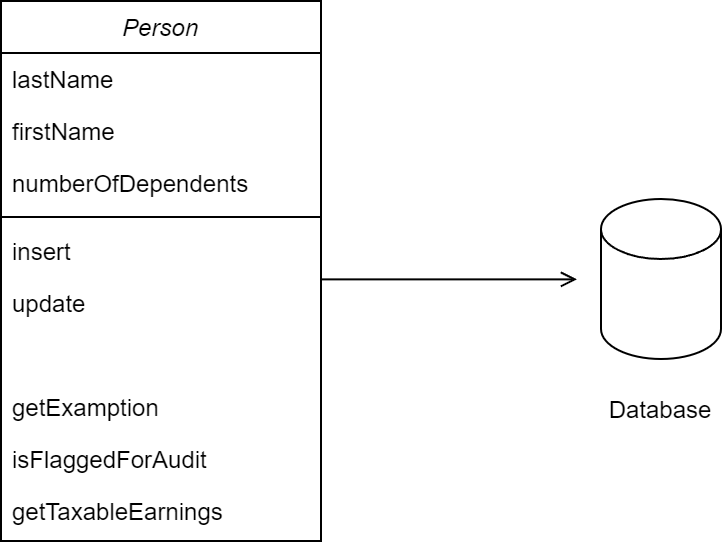
\includegraphics[width=0.6\textwidth]{ActiveRecord}
\end{figure}

The Active Record pattern is a~design pattern defined by Martin Fowler in his
book "Patterns of Enterprise Application Architecture"
\cite[p. 160]{fowler-patterns-2003} and is commonly used to represent database
records in an application.

The goal of the pattern is to encapsulate logic for interacting with the
database table into a~single object. Each instance of the object represents a
single record, and modifications made on it are then usually flushed with a
method call into the database. The base class also provides static methods for
CRUD (create, read, update, delete) operations and possibly additional business
logic.  

The main benefit of the Active Record pattern is a~simple and intuitive
interface for objects and tables. Modifications of the object can be made right
on the data in languages, which allow setters and getters on attributes, and
static methods provide a~simple gateway to work with the table. 

Limitations of the pattern come in the tight coupling between the application
and database logic, as the object instance is inherently tied to the database
representation. This makes it harder to test the implementation and often
requires additional abstraction or mocking. Additionally, the pattern does not
easily allow for the management of relations, so a~database schema with complex
relations might not be able to represent the data easily. 

\section*{Data mapper}

\begin{figure}[t]
    \caption{Data Mapper class diagram, recreated from Patterns of Enterprise Architecture}
    \centering
    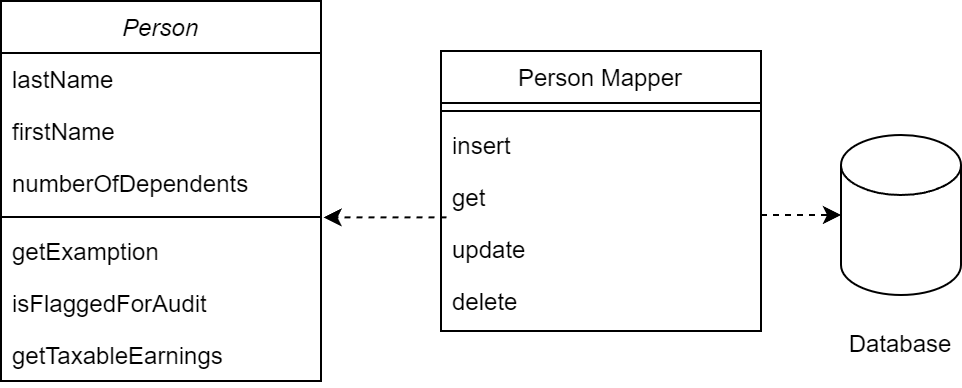
\includegraphics[width=0.8\textwidth]{DataMapper}
\end{figure}

The Data Mapper pattern, as described by Martin Fowler in his seminal work on
enterprise application architectures, provides a~clear separation between domain
models and their underlying data storage. This approach enables developers to
create complex and expressive domain models without being constrained by the
relational database schema or various storage options. By decoupling in-memory
representations from the data storage mechanisms, the Data Mapper pattern
promotes a~clean separation of concerns and enhanced flexibility in application
design \cite[p. 165]{fowler-patterns-2003}.

Distinguished from the Active Record pattern, the Data Mapper pattern ensures
that business logic and data access responsibilities remain separate. In this
approach, a~single entity represents the table or collection, while distinct
entities represent individual records. The Data Mapper serves as a~data access
layer that performs operations on the data storage representation without
creating any direct bindings between in-memory objects and the database. This
responsibility is solely managed by the Data Mapper, which takes care of any
objects that utilize it.

By limiting the responsibilities class must service and ensure that it is not
accountable for multiple unrelated tasks, the single responsibility principle
aims to create more straightforward and more maintainable classes. Consequently,
the Data Mapper pattern contributes to a~more robust and modular software
architecture that is easier to develop, maintain, and extend.

However, the Data Mapper pattern has drawbacks. One notable downside is the
increased complexity introduced by the additional layer of abstraction. This
added complexity could lead to a~steeper learning curve for developers
unfamiliar with the pattern, as well as the potential for increased development
time. Moreover, the mapping process between domain objects and the persistence
layer may introduce performance overhead, which can be a~concern for
applications with stringent performance requirements.

\setsecnumdepth{part}
\chapter{Framework selection}

Selecting the optimal framework for any project can be difficult with many parameters and options, and quite often, there are better options than the most popular. The JavaScript ecosystem is rich in choice, as throughout the years, many developers and companies have aimed to create packages in their image. Mainly due to this plethora of choices, there is a need for an overview, which would present advantages and disadvantages. However, only some frameworks can be reviewed; therefore, at least essential criteria need to be established. \par
The selected packages were selected for their support of TypeScript, with varying levels of compatibility, which will be shown in further detail later. Additional criteria considered were popularity and support as separate factors, leading to the inclusion of widely-used packages with currently limited support and development and lesser-known packages with solid support. \par
\section{Typescript support}
The primary selection criterion for the packages was TypeScript compatibility. Each package had to have at least a basic functionality working and typed, requiring only reasonable effort to integrate. The degree of support varies among the packages, and their level was also measured in comparison, but the base level was necessary to be considered.\par
The functionality considered essential is not easy to define either, but as the level of type support varied, the minimum settled on was package and connection setup and simple querying. The package had to have connection options typed, at least for primary usage, as listing all options for all connections is not necessary for most uses. Querying and updating database records is the most common activity for which ORMs and connection builders will be used, so the types they provide are some of the most useful. The result of a simple non-joined query on one table should be able to return exact and correct types, and an update of the record should also at least suggest the attributes which can be changed.\par
\section{Popularity and Support}
Popularity was inherently a factor in the selection of packages; if the package was known more, its likelihood of being found was smaller. We researched popularity in several ways; the primary source was searching by name and keyword ORM on the npm repository. Secondary sources were articles on ORM and database access in Node.js. The npm repository provides statistics about the packages listed on it, the most prominent being weekly downloads. The statistic is good for basic orientation but is not a great indicator of the exact number of users, as users can download the package multiple times, most packages are cached by third parties, which automatically download a version when it is released and many more ways, which skew the number. Additional input for popularity was the number of issues and stars the project currently holds on GitHub.\par
Support is a secondary attribute that is highly linked to popularity. Although all packages reviewed are open-source, only maintainers can merge code into the main branch or release versions onto the registry. If they are no longer active, the project effectively stops. While they can be released under a new name if the licence permits such a thing, no packages missing implementation into the benchmark have forks that would relieve the issues encountered. High-quality support is crucial for addressing issues, incorporating new features and compatibility with changes in underlying technologies.\par
\section{Implementation criteria}
Although some packages were initially selected for comparison, as previously mentioned, problems that needed to be more severe were encountered during their implementation into the included benchmarks. They will still be introduced, and the issues explained; however, they will only be included in comparisons within the basic summary.
\chapter{Ranking and Grading of the Frameworks}

This chapter outlines and explains the criteria for evaluating ORM and SQL query
builder packages chosen for the comparison. These criteria will be the core
points which will be considered, but other specific notes will be made about
each package. The main criteria were the level of TypeScript support, range of
compatible database management systems, popularity, support, documentation
quality, dependency count, and performance in different scenarios.

\section{Quantifiable Criteria}

The main section of the evaluation criteria focuses on technical aspects of the
frameworks, specifically their usage of TypeScript, support for different
databases, and difficulty composing queries. As these qualities are
quantifiable, they were given the highest priority in comparing the packages.

\subsection{TypeScript Support}

The quality and extent of TypeScript support vary among the packages, with some
offering better integration and type safety without the need for casts. In
contrast, others only provide basic typing or require result type definitions to
be written into each request, which amounts to the same behaviour as if the
result was cast. Such functionality often comes when the package initially
written for JavaScript is not rewritten in TypeScript but is only provided with
a \texttt{types} file, which specifies call signatures, but cannot provide other
assurances.

\subsection{Database Compatibility}

Wide database compatibility is necessary when working with a~large project that
may encompass many services or when choosing a~toolchain for a~team working with
dynamic technology stack, as the one database may not satisfy all the needs the
team might have, and building experience with multiple frameworks could be
considered unnecessary spending. Providing a~unified API over multiple databases
can be one of the benefits of query builders or object-relational mapping
frameworks.

\subsection{Flexibility and Performance}

Flexibility and performance are crucial in a~database access framework. Suppose
the package would restrict the ability to access the data, requiring roundabout
ways to deal with basic operations. In that case, there are better ways to
simplify development, just as if the framework creates excessively suboptimal
queries or adds excessive overhead. One of the requirements for a~comprehensive
ORM framework is the ability to support many use cases and represent and work
with many different data models. If ORM doesn't support possible use cases or
cannot represent commonly used database design patterns, it is lacking in some
ways compared to one that does.

Performance is often secondary when choosing an ORM framework, as quite often,
even frameworks adding significant overhead and creating suboptimal queries are
usually not noticeably slowing down the application. As the application grows,
the performance can become significantly more critical, and the resources needed
can be more expensive to scale. a~high-performing package can support this
growth by maintaining efficacy under load and effectively using its available
resources.

Performance was measured in multiple ways; the first metric was the execution
time of a~single query to measure the latency added by using the framework,
compared to using other frameworks or plain database drivers. Benchmarking this
way provides information about the amount of overhead the framework requires to
function, and if the connection pool is well initialized, connections are
assigned optimally, and data are correctly retrieved. The second benchmark run
repeats the test multiple times to eliminate any inconsistency that could occur
in a~single run.

\subsection{ECMAScript and CommonJS compatibility}
There are two different primary standards for JavaScript syntax, ECMAScript and
CommonJS. They primarily differ in how the inclusion of modules is written and
the mechanism of the module import. While CommonJS was dominant in the server
backend space for a~long time, however, ECMAScript modules are becoming
significantly more popular, with support added in Node.js, TypeScript and many
popular packages.

Combining packages from both ecosystems can still lead to problems. The best way
to support all possible combinations is to provide both types of dependency
declarations.

\subsection{Licence}
As developers consider integrating packages into their projects, it is crucial
to consider and understand the significance of licences governing their use.
Open-source software is often regarded as a~valuable resource, offering a~large
amount of reusable code and often the best solution. However, it is essential to
understand that open-source does not necessarily equate to unregulated use.
Licences still dictate the terms under which the package and its code can be
employed, modified and redistributed. Therefore, developers must examine the
licences of potential packages to ensure their intended use aligns with the
terms granted.

The most permissive licences allow for usage, modification and redistribution
with at most a~requirement to credit the original author/authors and don't
require the licensee to maintain the same licence in derivative works. Examples
of such permissive licences are \textit{MIT License} \cite{MITLicense} or
\textit{Apache License 2.0} \cite{ApacheLicense2}. These are generally preferable
for projects that demand flexibility in their use of the software.

While still free, the opposite side to the permissive licences are copyleft
licences, which impose more stringent requirements on the usage, especially
modifications and redistributions of the software. The primary example of such a
licence is \textit{GNU General Public License} \cite{GNUGPL}, which requires
derived works to be distributed under the same licence.

Since copyleft or other provisions might limit the usability of libraries such
as ORMs for many projects, it is necessary to include the licence as a~grading
criterion.

\section{Package Properties Criteria}

However, technical criteria are only some that should be considered when
selecting a~framework. Many of these factors are interconnected; often, success
in one is either caused by or preceded by doing well in others. For example,
while the popularity of the package can show the reliability and usability of
the package, it also often results in more issues being reported, and more
users are more likely to create community resources supplying or improving
official documentation.

\subsection{Popularity}

Popularity measures usage, as indicated by package downloads, the number of
issues, and the number of users on GitHub who have shown interest in the
repository. While all imperfect measures for absolute popularity, they help
compare popularity between packages by their relative difference. In the case
that the package usage requires multiple dependencies to be installed, for
example command line interface for development and runtime dependency, the
highest number is listed.

\subsection{Support}

The number of resolved and still open issues can be used to show popularity and
support of the project. With such a~metric, support can be measured; however,
more important than that are the patterns of behaviour which maintainers have
shown previously. If the release schedule is predictable, bugs and security
issues are fixed quickly, hesitant adopters can be assured that this pattern
will continue, and the framework is a~safe investment. On the contrary, a
project which is officially or probably no longer supported can be assumed to be
a wrong choice, as it cannot react to newly found errors and problems with
dependencies and might be unusable due to changes with TypeScript or Node.js
runtime.

\subsection{Dependencies}

As dependencies require maintenance due to their changes and vulnerable
versions, their amount should also be manageable. Otherwise, it might increase
the maintenance cost for the package and application size. Even though data
storage is less critical than previously, having a~more storage-conscious
package is still beneficial.

\subsection{Documentation Quality}

Documentation quality is critical for new adoption and onboarding for working
with the framework. It also cannot be measured with reasonable objectivity.
Perceived quality depends on language understanding and users’ previous
experience with the programming language and similar frameworks. Evaluation of
documentation will therefore summarize clarity, extensiveness and whether
features such as JSdoc annotations \cite{Typescript-jsdoc} which can be parsed
by IDEs are used to contain or link to the documentation.


The following chapters aim to provide a~comprehensive and in-depth analysis of
packages compared by evaluating each package by these comprehensive criteria
with additional added when.

\chapter{Benchmark database schema design}\label{ch:database}

\section{Introduction}
This chapter describes the database used for performance testing of the ORM and
query builder packages. The database is designed around imaginary data
collection about cats, their home domiciles and toys found within these houses,
and the toys' manufacturers. The database comprises six main entities -
\texttt{cat}, \texttt{cat colours}, colour \texttt{hex codes}, \texttt{houses},
\texttt{toys} and \texttt{toy producers}.

\section{Cat Entity}
The \texttt{cat} entity instances represent individual cats which we want to
monitor. Each has a unique identifier, name and date of birth, all of which are
nullable except for the identifier. This entity aims to represent the basic
database table and to verify the correct handling of the data type from
Postgres, as JavaScript Date time represents a moment, including time. In
contrast, the database entry would only contain the date. Additionally, the
\texttt{cat} entity uses big integer data type, and handling numbers beyond the
standard range allocated in JavaScript is tested. The \texttt{cat colour} and
\texttt{colour hex code} are two entities that represent the cat colour by its
name and by its hex code. The entities are intentionally split in this way to
use identifying relation - the primary key of the hex colour entity is also a
foreign key referencing the id of the cat colour entity.

\section{House and Toy Entities}
The \texttt{house} entity represents domiciles where the cats spend their time
at their behest. The relation must also account for ambitious cats using several
houses as their homes. The main aim is to test the difficulty of implementing
and using simple many-to-many relations. The only attribute that provides new
data type or behaviour is the simple \verb|has_dog| attribute, specified as a
Boolean. It is one of several attributes that test the frameworks' ability to
correctly type and convert the data recovered from the database.

The houses can be equipped with many toys for the cats to use. The relation
between houses and toys is modelled through a decomposition table which contains
attributes representing the number of the same toy in the house. While the
primary keys are the identifiers of the house and toy, the decomposition with
the amount, rather than several records with an additional identifier, is
designed to test the ability to insert a record if it does not exist or update
the value referencing its previous state. If more toys are purchased, the owner
of the house does not suddenly throw out all toys they already had; they will
add them to their current pile. This operation is often called \textit{upsert} -
a combination of update and insert, and some database engines, such as
CockroachDB, implement it explicitly under this name. PostgreSQL achieves it
using the \texttt{ON CONFLICT} statement in \texttt{INSERT} query. It also tests
the handling of composite primary keys, a standard paradigm in many databases.

\section{Toy Entity}
The \texttt{toy} entity purpose in testing is in numeric data type used in
\texttt{price} attribute and usage of additional column attributes such as
\texttt{CHECK} constraints or \texttt{DEFAULT} values in the column. Column
\texttt{naughty} is focused on commonly problematic strings in software
development, such as special Unicode characters, emojis and other issues that
could come up in handling data from the database, especially if the encoding is
not correctly handled. Toys producers host the JSON columns to test if it is
possible to use advanced JSON traversal and query operators provided in
PostgreSQL (and their equivalents in other database management systems).

\chapter{Benchmark Framework Design}

The benchmarking process was designed to compare the performance of various ORM
and SQL query builder packages. As such, it was important to ensure that the
benchmarking framework was developed in the same environment as the packages
themselves. To achieve this, the framework was implemented in TypeScript, the
same language used by the packages being tested.

The benchmarking framework had to be designed to accommodate errors that could
occur during development and testing of the packages. Additionally, it has to
support testing of multiple database schemas and allow for results to be
exported in a~variety of formats for further analysis. The resulting
benchmarking framework provides a~robust and comprehensive means of comparing
database access packages.

\section{Test Suite and Schema Separation}

The benchmarking framework was designed to support separation of tests into
multiple test suites, a~common practice with JavaScript test frameworks such as
Jest \cite{Jest} or Mocha \cite{Mocha}. Test suite separation allows for
organization of tests by subject and contains specifications about the database
schema and data expected to be executed. Input and output parameters must be
typed to test types support, and the framework should provide sufficient
functionality to avoid the need for casting.

The tests are expected to be run simultaneously with snapshots of the database
schema and should not interfere with data used by another test suite. As a
deliberate choice, this limits the scope of each test's modifications over the
database and data. However, it eliminates the need to reset the database to the
original state after each test suite, reducing the time it takes to run the
benchmark. However, such functionality should still be supported, as the
framework should allow for wider range of tests than is expected for
implementation.

\section{Database management}
As the framework operates strictly over a~database instance, the framework must
be able to perform maintenance operations. These include initializing the
database with its schema, seeding the database with test data and later tearing
down the schema and replacing it with a~different one, depending on which the
test suite requires.

\section{Test type and Error Handling}

The framework needs to support multiple tests to ensure the validity of any
results it produces. If performance is measured, multiple runs can reduce the
impact of statistical anomalies, which can occur due to the innumerable possible
external events.

Along with performance, the correctness of both query types, resulting runtime
types, and the result value are essential. As types are only visible before
compilation, and with typed test suite definitions TypeScript compiler would not
compile the code. Due to this restriction, even incorrect types from the
packages will need to be cast into their expected value. However, even just the
need for such modification means the package is insufficiently supporting type
definitions.

Resulting runtime types and values are validated using the node module
\texttt{node:assert} \cite{NodeAssert}, which provides assertion functions. It
is provided to function with testing frameworks such as mocha, which do not
offer verification functions. Included are even deep equality checking
functions. The main advantage, however, comes from being included in the Node.js
standard library, meaning that no additional package has to be included.

Returning an incorrect result is one of many ways the benchmark test can be
failed; the package can return an unexpected error, or the test is impossible to
perform. Both are fail-states, which the benchmark suite must account for with
error handling. One choice during the design process was that a~single failure
would mark the real test as failed, even though other iterations succeeded. If
the package caused the issue, that means the package is not reliable enough and
such problem needs to be marked. If the failure is caused by external issue, for
example database error, the test run can be repeated after triage.

\section{Multi-Framework support}

The benchmarking bootstrap is designed for sequential testing of multiple
packages. This design, rather than separate execution, allows for comprehensive
comparison under the same conditions, ensuring accurate results. As managing the
dependencies could prove problematic if packages had different dependencies
required, npm workspaces \cite{npmWorkspaces} were selected as a~project
structure. That way, top-level dependencies of the framework can be separated
from the individual implementations.

As each framework is initialized through its initialization method, abstraction
over the package itself must be created. The initialization also has to account
for delayed connection pool creation. Some packages only start the connection
once the first request is sent to limit the number of open connections for the
database. The database has a~limited amount of connections it can support, which
is one way to optimize its usage. The benchmark database can easily handle the
limited connections between the benchmarking framework and the individual
connections; however, it should still contain a~method for closing the
connection and destroying the context so subsequent frameworks can access the
same amount of resources.

\section{Reporters - Output options}

An integral part of the design was the inclusion of reporters. Reporters provide
an interface and implementation of multiple output options, enabling the results
to be saved and shown in various formats. Standard test frameworks utilize
reporters to make code coverage or detailed error stack inspectable. The
reporters can interpret the data in different formats with a~benchmarking
framework. The reporter interface has to be designed to be extensible, in order
to allow for the easy addition of other output options or data interpretations
in the future.


\setsecnumdepth{part}
\chapter{Conclusion}


\bibliographystyle{assets/iso690}
\bibliography{mybibliographyfile}

\setsecnumdepth{all}
\appendix

\chapter{Acronyms}
% \printglossaries
\begin{description}
	\item[PDA] Push-down automaton 
	\item[DFA] Deterministic finite automata
\end{description}


\chapter{Contents of enclosed medium}

%change appropriately

\begin{figure}
	\dirtree{%
		.1 readme.txt\DTcomment{the file with CD contents description}.
		.1 exe\DTcomment{the directory with executables}.
		.1 src\DTcomment{the directory of source codes}.
		.2 wbdcm\DTcomment{implementation sources}.
		.2 thesis\DTcomment{the directory of \LaTeX{} source codes of the thesis}.
		.1 text\DTcomment{the thesis text directory}.
		.2 thesis.pdf\DTcomment{the thesis text in PDF format}.
		.2 thesis.ps\DTcomment{the thesis text in PS format}.
	}
\end{figure}

\end{document}
